\documentclass{article}
\usepackage{graphicx}
\usepackage[spanish, es-tabla]{babel}
\renewcommand{\baselinestretch}{1.5}
\usepackage[backend=bibtex,sorting=none]{biblatex}
\bibliography{bibliography}
\usepackage[ruled,vlined]{algorithm2e}
\usepackage{algorithmic}



\begin{document}
		
	\begin{titlepage}
		\centering
		{
\includegraphics[width=0.2\textwidth]{logo}\par}
		\vspace{1cm}
		{\bfseries\LARGE Instituo Tecnológico de Oaxaca \par}
		\vspace{1cm}
		{\scshape\Large Ingeniería en Sistemas Computacionales  \par}
		\vspace{3cm}
		{\scshape\Huge Simulación de Difusión En Redes Sociales \par}
		\vspace{3cm}
		\vfill
		{\Large Autor: \par}
		{\Large José Ángel García García \par}
		\vfill
		{\Large Diciembre 2020 \par}
		\end{titlepage}
	
\tableofcontents
\newpage
	
\section{Introducción}
 
 \subsection{Planteamiento del problema}
 Las redes sociales son el medio de comunicación que predominan actualmente, se han incorporado a nuestras vida hasta un grado en el que no somos capaces de asumir que dependemos de ellas o que hacemos una gran inversión de tiempo en ellas, por más minimo que sea el tiempo por día, sumado semanalmente da un valor de tiempo elevado. Entonces podemos decir que las redes sociales son parte de nuestra vida, de nuestro día a día, es tan común, leer noticias, compartir información con contactos e inclusive comunicarse con nuestros familiares cercanos; lo hacemos a diario y ya no nos vemos como consumidores de una red social.
  
 Hoy en día el término \textit{red social} es muy empleado llamándose así a los diferentes sitios o páginas de internet que ofrecen registrarse a las personas y contactarse con infinidad de individuos a fin  de compartir contenidos, interactuar y crear comunidades sobre intereses similares: trabajo lecturas, amistad, juegos, relaciones amorosas, entre otros.

 En Boyd y Ellison, definieron a las redes sociales como "Las redes sociales son una estructura social que se puede representar en forma de uno o varios grafos, en los cuales, los nodos representan a individuos (a veces denominados actores) y las aristas, relaciones entre ellos. Las relaciones pueden ser de distinto tipo, como intercambios financieros, amistad, relaciones sexuales o rutas aéreas. También es el medio de interacción de distintas personas, como por ejemplo, juegos en línea, chats, foros, spaces, entre otros. Las redes sociales facilitan en gran medida esta interacción, pueden clasificarse en redes sociales personales, que agrupan a un conjunto de contactos y amigos con intereses en común, y redes sociales profesionales, redes que se centran más en la creación de contactos profesionales afines a cada usuario."\cite{definition:redsocial}. 
 
 Como sociedad que somos, nuestra forma de actuar y comportarnos está influenciada por otros individuos, es decir, existen individuos que influyen sobre otros para realizar determinadas acciones. La información, conocimiento, valores, tradiciones, culturas, etc., que surge mediante una red social es a tal grado que se crea una especie de tejido social. La identificación de los difusores más influyentes que maximizan la propagación de la información en las redes sociales es un problema de optimización clásico, llamado problema de maximización de influencia (IM).
   
 \subsection{Definición del sistema}
La información que viaja y fluye en una red social a través de diferentes medios puede ser: publicidad, publicaciones, fotos y vídeos, etc., se expande de forma exponencial, primeramente con ayuda de un pequeño grupo de personas influyentes; existen personas con un estatus de aceptación mayor que otras, es decir, personas líderes de opinión que gracias a estos, hacen que se propage la información entre los individuos haciendo que incremente el grado de difusión.

En este documento se plantea estudiar el comportamiento de la difusión de información. Exactamente se plantea que el sistema sea capaz de simular la sinergía del flujo de la información en las redes sociales. Un modelo de difusión razonable que pueda simular con precisión la propagación de información en las redes sociales es el paso clave para resolver eficazmente el problema de la maximización de influencia
 
\section{Diseño del Modelo}
 
 \subsection{Formulación del modelo}
  Una red social, como lo menciona Boyd y Elison se puede modelar como un gráfico con vértices que representan a los usuarios y bordes que representan los enlaces entre los usuarios. El proceso en cascada en la red se realiza bajo un modelo de difusión especificado.\\
 “El problema de IM se define como encontrar $k$ nodos semilla en la red como la fuente de  propagación de información de modo que, bajo la difusión especificada en el modelo, la escala  de la cascada se maximiza” \cite{cite:problemaIM}.
 
 Flaviano y Hernan A, mapearon la información difundida en las redes sociales en una  filtración óptima y presentaron un algoritmo, llamado influencia colectiva (IC), basado en la  conexión débil entre los nodos para identificar el conjunto mínimo de influenciadores. En base a  esta información, los autores aprovechan el comportamiento de los usuarios en redes reales,  incluidos Twitter, Facebook, APS y LiveJournal, y utilizan el algoritmo de CI para localizar  difusores influyentes. “Los resultados experimentales muestran que el conjunto óptimo de semillas es mucho más pequeño que el obtenido por otras medidas”\cite{cite:semillas}.
 
 La sinergia es un fenómeno omnipresente en los sistemas sociales. Muchos estudios han encontrado que “la sinergia aumenta la probabilidad de transmisión entre un par de nodos y promueve la propagación de explosiva”\cite{cite:sinergia}. Por ejemplo, en términos de información difundida en las redes sociales, un mensaje transmitido por un grupo de usuarios conectados es más creíble que un mensaje transmitido por un individuo, para incorporar esto conceptos se creó el modelo de difusión llamado modelo de cascada de tres pasos basado en sinergismo \textbf{(TSSCM)} basado en el análisis anterior y la teoría de la influencia de tres grados.
 
\subsection{Explicación del modelo}

Se define un gráfico no ponderado y no dirigido $G = (V,E)$, Donde $V$ es el conjunto de vértices y $E$ es el conjunto de aristas. El gráfico puede modelar una red social en línea, un nodo $v \in V$ Representa a un individuo en la red social y una ventaja e $(u, v) \in E$. TSSCM, suponen que el nodo u puede influir en el nodo $v$ solo si la distancia de $u$ a $v$ no es mayor que tres. Cuando u intenta activar $v$, la probabilidad de activación $\alpha(u, v)$ depende no solo del número de vecinos activados conectados a usted, pero también la profundidad de la cascada.\\

En TSSCM, suponemos que el nodo $u$ puede influir en el nodo $v$ solo si la distancia de $u$ a $v$ no es mayor que tres. Cuando $u$ intenta activar $v$, la probabilidad de activación $\alpha(u, v)$ depende no solo del número de vecinos activados conectados a $u$, sino también de la profundidad de la cascada $d(d = 1,2,3)$.


\begin{eqnarray}
	\alpha(u,v) = p(u,v)l(d) \\
	p(u,v) = 1 - (1 - \beta^{ 1 + \frac{m}{k-1} })\\
	l(d) = \frac{1}{d}(d = 1,2,3)
\end{eqnarray}


La ecuación $(2)$ indica que cuanto mayor es el valor de $\frac{m}{k - 1}$, cuanto mayor sea la tasa de sinergia. El modelo TSSCM se reduce al modelo clásico de la década para $d = 1$ y $m = 0$, donde $\alpha(u, v) = \beta$. Si $m > 0$, entonces $\alpha(u, v) > \beta$, Además, $k > 1$ para los nodos no hoja, por lo tanto, la capacidad sinérgica de cualquier vecino activado de un nodo activo es menor que la de sí mismo.\\

" Esta suposición se basa en la propagación de la enfermedad real, donde la probabilidad de que un nodo susceptible está infectado por un vecino directo infectado siempre es mayor que la probabilidad de infectarse por un vecino indirecto infectado ".\cite{cite:36}

Para $d > 1$, TSSCM funciona de la siguiente manera. Sea $S_o \subseteq V$ el conjunto de semillas. Todos los nodos $S_o$ se activan en el primer paso de tiempo. En los pasos en $0\leq t \leq 3$, $S_t \subseteq V $es el conjunto de nodos que se activan en el paso $t$. En el paso $t + 1$, cada nodo intenta activar su nodo $v\not\in S_t$ vecino con probabilidad $\alpha(u, v)$. Si dicha activación es exitosa, entonces $v$ cambia el estado de inactivo a activo y permanece en el estado activo. Cada nodo activado solo tiene una oportunidad de activar a sus vecinos durante el paso inmediatamente posterior a su activación inicial. El proceso en cascada anterior se repite hasta que no se puedan activar nodos en la red o $t = 3$. 

Como se muestra en la \ref{Fig:01}, en el paso $t$, el nodo $1$ es una semilla y los otros nodos están inactivos. Para el nodo $1$, no hay vecinos activos; así, $m = 0, \alpha(1,2) =, \alpha(1,3) =, \alpha(1,4) = 1 - (1 - \beta)^{1+\frac{0}{3-1}} = \beta$, lo que significa que el nodo $1$ activa a sus vecinos con probabilidad $\beta$. En el paso $t + 1$, el nodo $3$ es activado por el nodo $1$. Debido a que tiene un vecino activo, el nodo 3 activará a sus vecinos, el nodo $5$ y el nodo $6$, con una gran probabilidad $\alpha(1,5) = \alpha(1,6) = 1 - (1 - \beta)^{1+\frac{1}{2}}$. A diferencia de otros modelos de difusión, TSSCM acumula sinergia, es decir, los vecinos activos de un nodo activo cooperan para difundir información. Este fenómeno es común en los sistemas sociales reales, como la propagación de información y la invasión animal.

\begin{figure}[h]
	\centering
	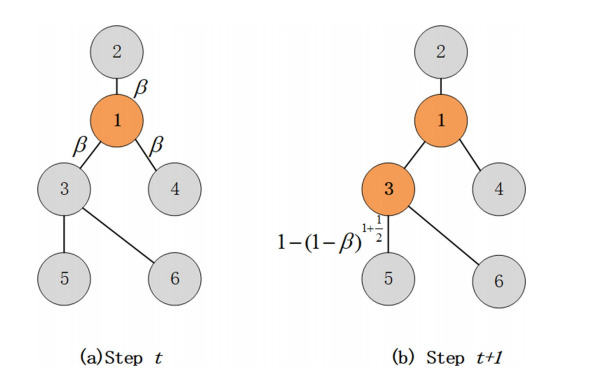
\includegraphics{Fig1.PNG}
	\label{Fig:01}
	\caption{Proceso del modelo TSSCM.}
\end{figure}

\textbf{Problema de maximización de influencia bajo TSSCM}\\

Dado un conjunto de semillas $S$, usamos $\sigma_{TSSCM}(S)$ para representar la influyente de $S$, que puede cuantificarse como el número de nodos activados bajo $TSSCM$ cuando finaliza el proceso de propagación. \\
El problema de IM bajo $TSSCM$ se define como: \\

\textbf{Definición 1} Dada una red $G = (V, E)$, el problema de mensajería instantanea en $TSSCM$ tiene como objetivo encontrar el subconjutno de $S^* \subseteq V, |S^*|= K$ tal que: 
\begin{equation}
	\centering
	S^* = arg_smax\sigma_{TSSCM}(S)
\end{equation}
Kempe y col \cite{cite:12} han demostrado que el problema de IM es NP-hard utilizando el problema de máxima cobertura. Basados en esta prueba, consideramos un método de reducción similar y probamos que el problema de IM bajo TSSCM es NP-hard.

La solución óptima del problema de maximización de influencia en TSSCM puede ser aproximada por los codiciosos algoritmo,  $Greedy(G, \sigma_{TSSCN}(S), k)$, como se muestra en el algoritmo \ref{algoritmo:Algoritmo 1}.\\

\begin{algorithm}[h]
	\label{algoritmo:Algoritmo 1}
	\KwIn{$G$ red; $K$ tamaño de el conjunto de semillas}
	\KwOut{Conjunto de semillas $S$ }
	\caption{Algoritmo 1 $Greedy(G, \sigma_{TSSCN}(S), k)$}
	\textbf{Inicializa } S = 0\\
	\begin{algorithmic}
	 \WHILE {$|S| < K$}
	 \STATE $\textbf{select} v = arg max_{v \in V(\sigma(S \cup v) - \sigma(S))}$
	 \STATE $S = S \cup v	$
	 \ENDWHILE
	 \RETURN $S$;
	\end{algorithmic}
\end{algorithm}


Para optimizar la función global del problema de MI, Flaviano Morone \cite{cite:30} la información mapeada se diseminó asintóticamente sobre la percolación óptima y propuso otra medida de centralidad topológica llamada CI, que se define como \\
\begin{equation}
	\centering
	CI_l(i) = (K_i - 1) \sum_{j \in Ball (i,l)} (K_j-1)
\end{equation}
Donde $K_i$ es el grado del nodo $i$ y $Ball (i,l)$ denota el conjunto de nodos a una distancia $l$ del nodo $i$.\\

El $CI$ anterior no considera la tasa de propagación entre dos nodos vinculados. Sin embargo, en el proceso de difusión de información real, un nodo recibe información transmitida por otros nodos vecinos con una cierta probabilidad. Claramente, un algoritmo realista y eficiente para la asignación óptima de recursos debe considerar tanto las características topológicas como los detalles de la dinámica; además, la propagación debe maximizarse dentro de un período de tiempo limitado. \\
Dado que $TSSCM$ es inherentemente probabilístico, propusimos una medida, llamada influencia colectiva de tres capas con sinergismo $(CI\_TLS)$, que incorpora la formulación de $CI$ y la dinámica de difusión con sinergismo. \\

Para nodo $i, l(i,v)$ denota la distancia más corta de $i$ a $v$. 
La influencia que se extiende del nodo $i$ se limita a un conjunto de nodos que consta de los nodos a una distancia $l$ de $i, L(i,l) = {v|l(i,v) = l, v \in V}$. Nosotros podemos asignar al nodo $i$ el $CI\_TLS$ mediante:
\begin{eqnarray}
	CI_TLS(i) = (K_i - 1) \sum_{v \in L(i,l)} (l = 1,2,3)\\
	\sigma(i,v) = 1 - \prod_{u \in L(i,l-1)} (1-\sigma(i,u)\alpha(u,v))\\
   A_{uv} = 1
\end{eqnarray}
Donde $\alpha(u,v)$ es la probabilidad de activación definida en, $\sigma(i,v)$ es la probabilidad final de activación del nodo $v$ por el nodo $i$ que obtenido mediante el calculo recursivo de la influencia de propagación. \\
El $CI\_TLS$ de un nodo contiene una rica información topológica y dinámica de propagación, que puede decirnos más sobre los roles de los nodos en la red que una medida que considera solo un aspecto

\begin{table}[h]
	\begin{center}
		\begin{tabular}{| c | c |}
			\hline
			\textbf{Variable} & \textbf{Descripción} \\ 
			\hline
			$\beta$ & Probabilidad de propagación basica \\
			$m$ & Número de vecinos activados conectados a una $u$\\
			$k$ & El grado del nodo $u$\\
			$\alpha(u,v)$ & Probabilidad de activación de algún nodo\\
			$p(u,v)$ & Sinergía del nodo\\
			$l(d)$ & Información en descomposición Ratio\\
			$\sigma(i,v)$ & Probabilidad de activación final del nodo $v$ por el nodo $i$ \\
			$CI$\_$TLS(i)$ & Suma que contiene las contribuciones de los nodos cuya distancia a $i$ es menor a 3\\
			\hline
		\end{tabular}
		\caption{Las variables utilizadas en el modelo TSSCM.}
		\label{tab:TablaVariables}
	\end{center}
\end{table}

\newpage
\section{Recolección de Datos}
 Los datos se pueden obtener de dos diferentes fuentes: 
 \begin{itemize}
 	\item[$1$] Internet\\ 
 	Basicamente se proprociona una pagina web de la cual se puende obtenerdiferentes datos. Dicha dirección se puede encontrar en \cite{data:01} 
 	\item[$2$] Experimentos\\
 	Se plantea obtener datos mediante la interacción de contactos mediante una red social, en la que a partir de una publicación pueda obtener los datos solicitados. 
 	De momento, veo viable usar Instragram, Facebook y LinkedLn para hacer los correspondientes experimentos.
 \end{itemize}
 \subsection{Recolección}
 	Aquí explicaré cómo hice la recolección a detalle. 
 \subsection{Análisis de Datos}	
	Aquí los datos ya recolectados.
	
\section{Construcción del Modelo}
	Aquí explicaré la programación
\section{Validación}
	Aquí verificaré el modelo ya simulado
\section{Conclusiones}
	Aquí finalizaré cómo fue el trabajo.
	
\section{Referencias}

\printbibliography

\end{document}